% Provenance (never printed): see sources/outline_sources.md (Year 2: Hadean, Archean and
% Proterozoic; early crust and greenstone belts; the oxygenation of the atmosphere; snowball
% Earth). Eons and eras from the ICS chart; greenstone belts, TTG and cratons after Cawood and
% others (2018) and Smithies and others (2019); komatiite liquidus after Sossi and O'Neill (2016),
% Pierru and others (2022) and Asimow (2022); the Archean air and the GOE after Catling and Zahnle
% (2020) and Luo and others (2016); the boring billion after Lyons and others (2021); snowball
% Earth after Hoffman and others (2017). The energy-balance model, the komatiite line and the CO2
% build-up from figdata/bachelor-2/precambrian.py; exercise and problem values in the Book 4
% scratch calculator calc/ch18.py.
\chapter{The Precambrian Earth}\label{ch:b2:precambrian-earth}

The first shelly fossils appear in rocks about 540 million years old. Everything before them, from
the birth of the Earth \qty{4567}{Ma} ago, is the Precambrian: seven-eighths of the planet's
history. In that time the Earth built the cores of its continents, filled its air with oxygen,
and at least twice froze over from the poles to the equator, with ice sheets reaching the sea
in the tropics. This chapter reads those four billion years in the rocks that survive from them,
and puts numbers on three of their puzzles: why the oldest lavas were so hot, how a frozen
planet can thaw, and how the young Earth stayed warm under a dim Sun.
% ledger: ics:base.Hadean, ics:base.Phanerozoic, hoffman17:cryochrons

\begin{recall}
\textbf{From the school volumes}: the age of the Earth; the eons on the geological time scale;
the young Sun's luminosity law and the \omterm{def:b2:precambrian-earth:faint-sun}{faint young Sun problem}; the primitive atmosphere;
stromatolites, \omterm{def:b2:precambrian-earth:bif}{banded iron formations}, the \omterm{def:b2:precambrian-earth:goe}{Great Oxidation Event} and red beds; \omterm{def:b2:precambrian-earth:craton}{cratons};
radiogenic heat in the past. \textbf{From the Year 1 volume}: zircon and its U--Pb ages,
closure temperature; radiogenic heat production of the four isotopes; outgoing longwave
radiation and the global mean insolation $S_0/4$; chronostratigraphic units.
\textbf{From earlier chapters}: the \omterm{def:b2:mantle-melting:tp}{mantle potential temperature} and the adiabat
(\cref{ch:b2:mantle-melting}); the liquidus and \omterm{def:b2:magmatic-differentiation:crystallisation}{fractional crystallisation} of olivine
(\cref{ch:b2:magmatic-differentiation}); granite types (\cref{ch:b2:crustal-melting});
\omterm{def:b2:wilson-cycle:supercontinent}{supercontinents} (\cref{ch:b2:wilson-cycle}). Oxidation and reduction belong to the chemistry
books, and the first eukaryotes and photosynthesis to the biology books.
\end{recall}

\section{Three eons before the fossils}\label{sec:b2:precambrian-earth:eons}

\begin{definition}[Hadean, Archean, Proterozoic]\label{def:b2:precambrian-earth:eons}
The time before the Phanerozoic is divided into three eons. The \emph{Hadean}\index{Hadean}
runs from the formation of the Earth, \qty{4567}{Ma} ago, to $4031 \pm \qty{3}{Ma}$; the
\emph{Archean}\index{Archean} from $4031$ to \qty{2500}{Ma}; the
\emph{Proterozoic}\index{Proterozoic} from 2500 to \qty{538.8}{Ma}, the base of the Cambrian.
Together they are informally called the Precambrian.
\end{definition}
% ledger: ics:base.Hadean, ics:base.Archean, ics:base.Proterozoic, ics:base.Phanerozoic

The \omterm{def:b2:precambrian-earth:eons}{Archean} is cut into four eras, the Eoarchean (4031 to \qty{3600}{Ma}), Paleoarchean (3600
to 3200), Mesoarchean (3200 to 2800) and Neoarchean (2800 to 2500); the \omterm{def:b2:precambrian-earth:eons}{Proterozoic} into three,
the Paleoproterozoic (2500 to \qty{1600}{Ma}), Mesoproterozoic (1600 to 1000) and
Neoproterozoic (1000 to 538.8). Two Neoproterozoic periods matter below, the Cryogenian, 720 to
\qty{635}{Ma}, and the Ediacaran, 635 to \qty{538.8}{Ma}.
% ledger: ics4:archean-eras, ics4:proterozoic-eras

\begin{omfigure}
\centering
% ledger: ics:base.Hadean, ics:base.Archean, ics:base.Proterozoic, ics:base.Phanerozoic, ics4:archean-eras, ics4:proterozoic-eras, wilde01:4404, bowring99:acasta, cz20:impacts, allwood06:spc, cawood18:transition, gumsley17:goe, luo16:goe, hoffman17:earlier, earle:bif, lyons21:boring, hoffman17:ages, asimow22:komatiite
\begin{tikzpicture}[x=-3.4cm, y=1cm, font=\scriptsize]
% eons
\fill[icsHadean] (4.567,0) rectangle (4.031,0.5);
\fill[icsArchean] (4.031,0) rectangle (2.5,0.5);
\fill[icsProterozoic] (2.5,0) rectangle (0.5388,0.5);
\fill[icsPhanerozoic] (0.5388,0) rectangle (0,0.5);
\node[text=white] at (4.299,0.25) {Hadean};
\node[text=white] at (3.27,0.25) {Archean};
\node[text=white] at (1.52,0.25) {Proterozoic};
\node at (0.27,0.25) {Phan.};
% eras
\foreach \a/\b/\c in {4.031/3.6/35, 3.6/3.2/55, 3.2/2.8/35, 2.8/2.5/55}
  \fill[icsArchean!\c] (\a,-0.45) rectangle (\b,0);
\foreach \a/\b/\c in {2.5/1.6/35, 1.6/1.0/55, 1.0/0.5388/35}
  \fill[icsProterozoic!\c] (\a,-0.45) rectangle (\b,0);
\foreach \x/\l in {3.8155/Eo, 3.4/Paleo, 3.0/Meso, 2.65/Neo, 2.05/Paleo, 1.3/Meso, 0.769/Neo}
  \node at (\x,-0.225) {\l};
% axis
\draw (4.6,-0.6) -- (0,-0.6);
\foreach \t in {0,0.5,...,4.5} {
  \draw (\t,-0.6) -- (\t,-0.7);
  \node[anchor=north] at (\t,-0.7) {\pgfmathprintnumber[fixed, precision=1]{\t}};
}
\node[anchor=north, font=\small] at (2.3,-1.05) {time before present (billion years)};
% row A
\fill[omDef] (4.404,0.85) circle (2pt);
\node[anchor=west, text=omDef] at (4.404,0.85) {oldest zircon};
\fill[omMeth] (3.43,0.85) circle (2pt);
\node[anchor=west, text=omMeth] at (3.43,0.85) {first stromatolites};
\draw[red!60!black, line width=3pt] (2.4,0.85) -- (1.8,0.85);
\node[anchor=west, text=red!60!black] at (1.8,0.85) {banded iron formations};
% row B
\fill[omDef] (4.03,1.5) circle (2pt);
\node[anchor=west, text=omDef] at (4.03,1.5) {oldest rocks};
\draw[black!70, line width=3pt] (3.2,1.5) -- (2.5,1.5);
\node[anchor=south, text=black!80] at (2.85,1.6) {change of tectonic style};
\draw[omProp, line width=3pt] (1.8,1.5) -- (0.8,1.5);
\node[anchor=south, text=omProp] at (1.3,1.6) {``boring billion''};
% row C
\draw[black!60, line width=2pt, densely dashed] (4.2,2.25) -- (3.5,2.25);
\node[anchor=south, text=black!70] at (3.85,2.35) {late heavy bombardment? (debated)};
\draw[omThm, line width=3pt] (2.43,2.25) -- (2.06,2.25);
\node[anchor=west, text=omThm] at (2.06,2.25) {Great Oxidation Event};
% row D
\fill[blue!60!black] (2.4,3.0) circle (2pt);
\node[anchor=east, text=blue!60!black] at (2.4,3.0) {first snowball Earth};
\fill[omThm] (0.8,3.0) circle (2pt);
\node[anchor=east, text=omThm] at (0.8,3.0) {second rise of oxygen};
% row E
\fill[orange!80!black] (1.9,3.7) circle (2pt);
\node[anchor=east, text=orange!80!black] at (1.9,3.7) {last common komatiites};
\draw[blue!60!black, line width=3pt] (0.717,3.7) -- (0.635,3.7);
\node[anchor=east, text=blue!60!black] at (0.717,3.7) {Cryogenian snowball Earths};
% row F
\fill[omMeth] (0.57,4.4) circle (2pt);
\node[anchor=east, text=omMeth] at (0.57,4.4) {first large fossils (Ediacaran)};
\end{tikzpicture}
\par\smallskip{\small The Precambrian on one line. The eons and, in lighter tints, their eras
(Eo-, Paleo-, Meso- and Neoarchean; Paleo-, Meso- and Neoproterozoic) are those of the
International Chronostratigraphic Chart; the events are placed at the ages quoted in the text.
The ``last common \omterm{def:b2:precambrian-earth:greenstone}{komatiites}'' are the aluminium-undepleted ones; younger, rarer kinds exist.}
\end{omfigure}

\subsection*{The Hadean: minerals without rocks}

No rock survives from the \omterm{def:b2:precambrian-earth:eons}{Hadean}, only minerals. The oldest is a grain of zircon from the Jack
Hills of Western Australia, $4404 \pm \qty{8}{Myr}$ old, washed out of an older rock and laid
down in a conglomerate some three billion years ago. Its composition, and that of its
neighbours, was read by its discoverers as evidence that a crust of continental type and
liquid water already existed \qty{4.4}{Gyr} ago, some 160 million years after the Earth
formed. The oldest dated rocks, the Acasta gneisses of north-western Canada, are 4.00 to
\qty{4.03}{Ga} old, close to the base of the \omterm{def:b2:precambrian-earth:eons}{Archean}.
% ledger: wilde01:4404, wilde01:zircon, uw14:jack-hills, bowring99:acasta

The young Earth was struck by large bodies, as \cref{ch:b2:planet-formation-meteorites}
described. The last impact large enough to vaporise
the whole ocean is estimated to have happened about \qty{4.3}{Ga} ago. A later ``late heavy
bombardment'', a burst of impacts between about 4.2--4.0 and \qty{3.5}{Ga} inferred from the
ages of lunar rocks and of shocks in \omterm{def:b2:planet-formation-meteorites:fall-find}{meteorites}, has been proposed; many dispute that it was a
distinct event at all, and either way it would probably not have sterilised the Earth.
% ledger: cz20:impacts

\section{The Archean crust}\label{sec:b2:precambrian-earth:archean}

\subsection*{Greenstone belts and komatiites}

The \omterm{def:b2:precambrian-earth:eons}{Archean} crust that survives is made of two kinds of terrain, side by side: large bodies of
grey, sodium-rich granitic gneiss, and narrower belts of altered volcanic and sedimentary rock.

\begin{definition}[Greenstone belt; komatiite]\label{def:b2:precambrian-earth:greenstone}
A \emph{greenstone belt}\index{greenstone belt} is a belt of mafic and ultramafic volcanic rocks,
with sediments, metamorphosed at low grade (the green comes from chlorite, actinolite and
epidote), lying between bodies of granitoid in \omterm{def:b2:precambrian-earth:eons}{Archean} and some \omterm{def:b2:precambrian-earth:eons}{Proterozoic} terrains. A
\emph{komatiite}\index{komatiite} is an ultramafic lava, far richer in MgO than basalt,
erupted as a liquid; its olivine typically grows in long, thin blades, the
\emph{spinifex} texture, as the top of the flow cools fast.
\end{definition}
% ledger: cawood18:dome-keel, so16:liquidus, pierru22:komatiite

\begin{omfigure}
\centering
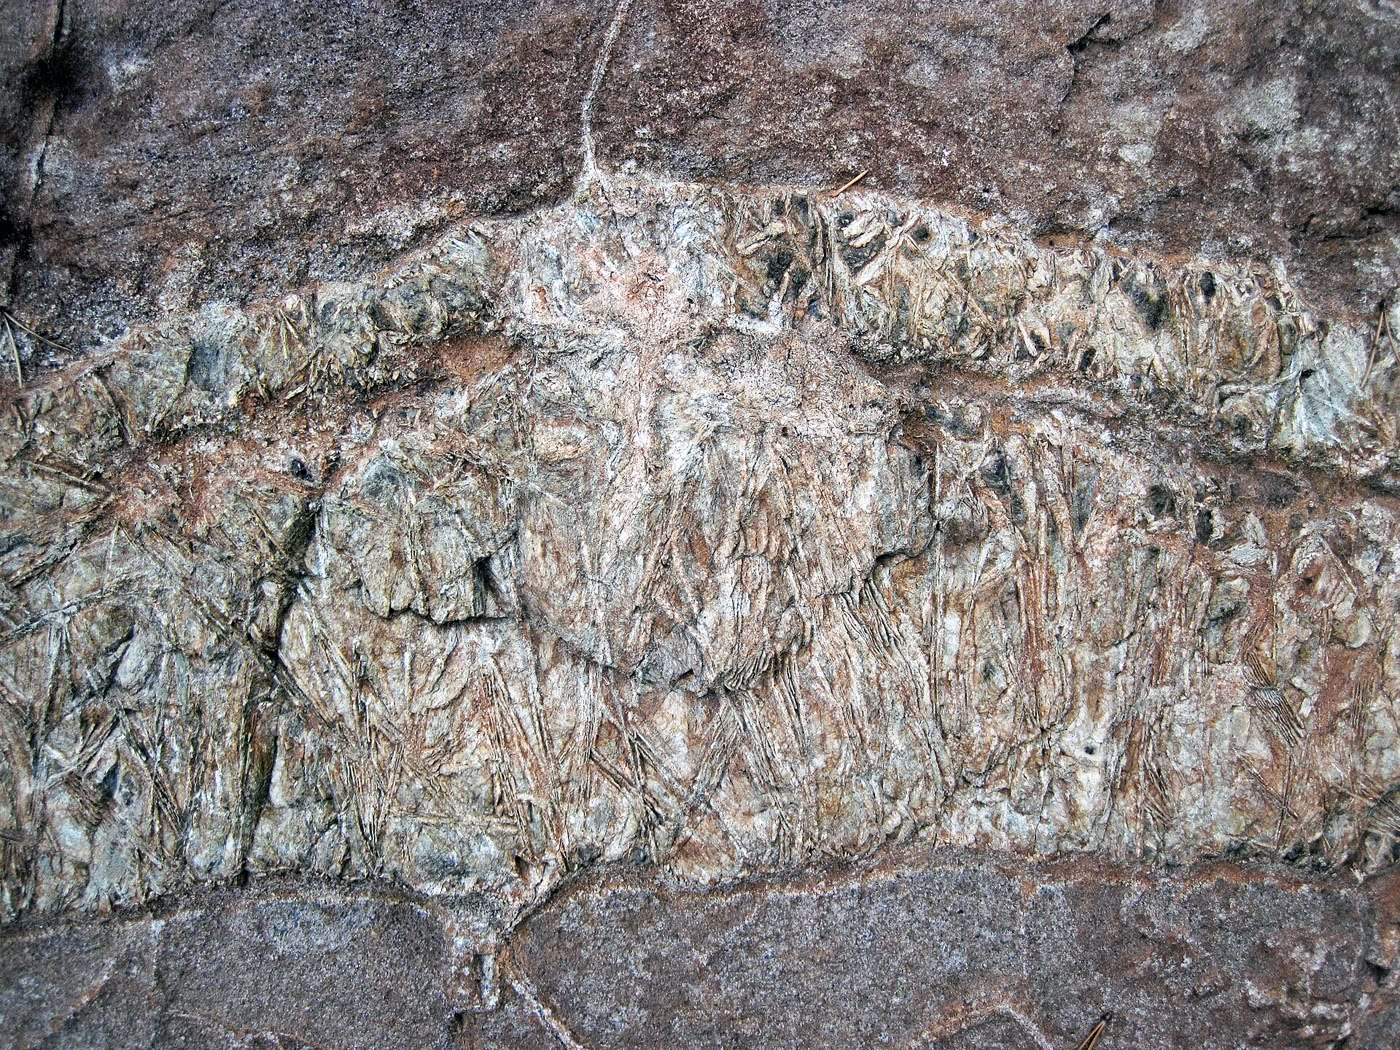
\includegraphics[width=0.66\linewidth]{images/book4/b2-18-spinifex-komatiite.jpg}
\par\smallskip{\small Spinifex texture in a \omterm{def:b2:precambrian-earth:greenstone}{komatiite} flow, Pyke Hill, Ontario, part of a
Neoarchean \omterm{def:b2:precambrian-earth:greenstone}{greenstone belt} about 2.71 billion years old: blades of olivine, now altered,
grew across the cooling top of the flow. Photograph James St.~John, CC~BY~2.0 (Wikimedia
Commons).}
\end{omfigure}

\omterm{def:b2:precambrian-earth:greenstone}{Komatiites} contain up to \qty{34}{\percent} MgO, against 10 to \qty{13}{\percent} in the primary
basalts of today's ridges, and they are almost confined to the old Earth: the aluminium-depleted
kind is found only in rocks older than \qty{2.8}{Ga}, the aluminium-undepleted kind until about
\qty{1.9}{Ga}, and only a rare aluminium-enriched kind is as young as \qty{90}{Myr}. A melt
that rich in magnesium is very hot, and, as for the basalts of
\cref{ch:b2:magmatic-differentiation}, the first mineral to crystallise from it is olivine,
whose share in the liquid fixes the temperature.
% ledger: pierru22:komatiite, asimow22:komatiite

\begin{proposition}[The komatiite thermometer]\label{prop:b2:precambrian-earth:liquidus}
For a melt in equilibrium with olivine at atmospheric pressure, the liquidus temperature rises
nearly linearly with the MgO content of the melt. Through two experiments $(m_1, T_1)$ and
$(m_2, T_2)$,
\[
  T_{\text{liq}}(m) = T_1 + s\,(m - m_1), \qquad s = \frac{T_1 - T_2}{m_1 - m_2} .
\]
Melting experiments on two \omterm{def:b2:precambrian-earth:greenstone}{komatiites}, $\qty{32.2}{\percent}$ MgO at \qty{1616}{\celsius} and
$\qty{23}{\percent}$ at \qty{1450}{\celsius}, give $s = \qty{18.0}{\celsius}$ per per cent of
MgO.
\end{proposition}
% ledger: so16:liquidus, helz98:glass-thermometer

\begin{proof}
Olivine is a solid solution of forsterite and fayalite, much richer in magnesium than the melt
it grows from. As the melt cools, olivine takes magnesium out of it, and the temperature at
which the melt is just saturated in olivine falls with its MgO content. Experiments show that
over the range of a given family of melts the fall is close to linear, so that the line through
two experiments interpolates between them; $s = (1616 - 1450)/(32.2 - 23) = 166/9.2 = 18.04$.
\end{proof}

The coefficient is not special to \omterm{def:b2:precambrian-earth:greenstone}{komatiites}. Glasses quenched from the lava of Kilauea,
calibrated in the same way, change by \qty{3}{\celsius} for \qty{0.15}{\percent} of MgO, that
is \qty{20}{\celsius} per per cent. Extending the \omterm{def:b2:precambrian-earth:greenstone}{komatiite} line down to a primary ridge basalt
with \qty{12}{\percent} MgO thus gives its liquidus within a few tens of degrees: $1616 -
18.0\times20.2 \approx \qty{1252}{\celsius}$. The hottest \omterm{def:b2:precambrian-earth:greenstone}{komatiite} liquids were therefore
some \qty{360}{\celsius} hotter than the melts that feed today's ridges, and the figure below
shows the line.
% ledger: helz98:glass-thermometer, so16:liquidus, pierru22:komatiite
% values: slope 18.043, T_morb12 1251.5, dT_kom_morb 364.5 (precambrian.py)

\begin{omfigure}
\centering
\begin{tikzpicture}
\begin{axis}[omrecord, width=0.72\linewidth, height=6cm, xmin=8, xmax=35, ymin=1150, ymax=1700,
  xlabel={MgO in the melt (\unit{\percent} by mass)}, ylabel={liquidus at 1 atm (\unit{\celsius})},
  xtick pos=bottom, ytick pos=left, clip=false,
  y tick label style={/pgf/number format/1000 sep={}}]
% computed in figdata/bachelor-2/precambrian.py part kom; ledger: so16:liquidus, pierru22:komatiite
\fill[omProp!15] (axis cs:10,1150) rectangle (axis cs:13,1700);
\addplot[black, line width=1.1pt] table[x=MgO, y=T] {figdata/out/bachelor-2-precambrian-kom.dat};
\addplot[only marks, mark=*, mark size=2.4pt, omThm] coordinates {(32.2,1616) (23,1450)};
\node[anchor=north west, font=\scriptsize, text=omThm] at (axis cs:32.2,1612) {Barberton};
\node[anchor=north west, font=\scriptsize, text=omThm] at (axis cs:23,1446) {Munro};
\node[anchor=south, font=\scriptsize, text=omProp, align=center] at (axis cs:11.5,1560)
  {primary\\ridge basalts};
\draw[densely dashed] (axis cs:12,1150) -- (axis cs:12,1251.5) -- (axis cs:8,1251.5);
\draw[densely dashed] (axis cs:32.2,1150) -- (axis cs:32.2,1616);
\draw[<->, omDef, thick] (axis cs:27,1251.5) -- (axis cs:27,1616);
\draw[densely dotted] (axis cs:12,1251.5) -- (axis cs:27,1251.5);
\draw[densely dotted] (axis cs:27,1616) -- (axis cs:32.2,1616);
\node[anchor=east, font=\scriptsize, text=omDef] at (axis cs:26.7,1330) {about \qty{360}{\celsius}};
\end{axis}
\end{tikzpicture}
\par\smallskip{\small The \omterm{def:b2:precambrian-earth:greenstone}{komatiite} thermometer: the line through the liquidus temperatures
measured on two \omterm{def:b2:precambrian-earth:greenstone}{komatiites} (dots), extended to the 10 to \qty{13}{\percent} MgO of the primary
basalts of today's ridges (band). The extension rests on the similar slope of basaltic melts.}
\end{omfigure}

Hotter lava does not mean a mantle hotter by the same amount. \omterm{def:b2:precambrian-earth:greenstone}{Komatiites} probably rose in
plumes, as the hottest basalts of today do at Hawaii, where the potential temperature is up to
about \qty{200}{\celsius} above the $1350 \pm \qty{50}{\celsius}$ of the ambient mantle. And
they formed by large degrees of melting, at greater depth. They are commonly thought to have
formed in a mantle 200 to \qty{300}{K} warmer than today's; an alternative view holds that
\omterm{def:b2:precambrian-earth:greenstone}{komatiites} were wet \omterm{def:b2:magma-emplacement:magma}{magmas}, formed at temperatures not much higher than the surrounding
mantle. Either way, the \omterm{def:b2:precambrian-earth:eons}{Archean} mantle was hotter, and the school
volumes gave one reason: 3 billion years ago the four radioactive isotopes released more than
twice today's heat (\cref{exo:b2:precambrian-earth:2}).
% ledger: asimow22:komatiite, pierru22:komatiite, so16:liquidus

\subsection*{TTG and the dome-and-keel pattern}

The grey gneisses between the \omterm{def:b2:precambrian-earth:greenstone}{greenstone belts} are not granites of the kind that
\cref{ch:b2:crustal-melting} described.

\begin{definition}[Tonalite--trondhjemite--granodiorite suite]\label{def:b2:precambrian-earth:ttg}
The \emph{tonalite--trondhjemite--granodiorite suite}\index{tonalite--trondhjemite--granodiorite
suite} (TTG) is the family of sodium-rich, potassium-poor granitoids --- tonalites,
trondhjemites (tonalites poor in mafic minerals) and granodiorites --- that makes up most of
the \omterm{def:b2:precambrian-earth:eons}{Archean} continental crust. Most of them formed by \omterm{def:b2:mantle-melting:melting}{partial melting} of hydrated basaltic
crust.
\end{definition}
% ledger: smithies19:ttg, cawood18:ttg

Much of the volume of today's continental crust had formed by the end of the \omterm{def:b2:precambrian-earth:eons}{Archean}, largely
as TTG. Some TTG carry trace-element signatures long read as melting at more than
\qty{50}{km} depth, a pressure not reached in younger continental crust, and these readings
weigh in the debate on when plate tectonics began; a 2019 study argued that those signatures
come instead from melts of the mantle, and that the common TTG formed at
depths no greater than the \qty{40}{km} of an ordinary continental crust today. Late in the
\omterm{def:b2:precambrian-earth:eons}{Archean}, between about 3.0 and \qty{2.5}{Ga}, the granitoids of most \omterm{def:b2:precambrian-earth:craton}{cratons} change from TTG
to potassium-rich granites, the sign of a thicker crust being melted again.
% ledger: smithies19:ttg, cawood18:ttg

In the eastern Pilbara of Australia, in Zimbabwe and in southern India, the two terrains draw a
striking pattern on the map. Rounded domes of granitoid are framed by synclinal keels of greenstone whose layers dip and face away from the domes. The domes are
thought to have risen as \omterm{def:b2:magma-emplacement:ascent}{diapirs}, light granitic crust rising through a thick, dense pile of
lavas that sank between them. In the Pilbara this doming went on for hundreds of millions of
years and stopped about \qty{3.1}{Ga} ago, after which the structures become linear, like those
of younger \omterm{def:b2:alpine-orogen:orogen}{orogens}.
% ledger: cawood18:dome-keel

\begin{omfigure}
\centering
\begin{tikzpicture}[x=0.95cm, y=0.95cm, font=\scriptsize]
% schematic, after the description in cawood18:dome-keel
\fill[lith basalt] (0,0) rectangle (12,7);
\draw (0,0) rectangle (12,7);
\foreach \cx/\cy/\rx/\ry in {2.4/4.7/1.7/1.4, 7.2/5.0/2.0/1.4, 4.6/1.6/1.9/1.1, 10.0/2.0/1.4/1.3}
  \filldraw[lith granite, draw=black, thick] (\cx,\cy) ellipse ({\rx} and {\ry});
% strike and dip in the greenstone, each dipping away from the nearest dome
% (positions and strikes from the outward normals of the ellipses, computed by hand)
\foreach \px/\py/\st in {3.9/5.99/309, 0.9/5.99/231, 0.9/3.41/129, 2.4/2.88/90, 4.52/4.7/0,
    9.62/5.0/0, 8.91/6.29/305, 5.49/6.29/235, 8.91/3.71/55, 5.49/3.71/125,
    6.92/1.6/0, 4.6/3.12/270, 2.28/1.6/180, 6.24/0.53/60,
    10.0/3.72/270, 11.29/0.78/47, 8.18/2.0/180, 11.29/3.22/313}
  \pic at (\px,\py) {strikedip={\st}{}};
\node[fill=white, inner sep=1.5pt] at (2.4,4.7) {TTG dome};
\node[fill=white, inner sep=1.5pt] at (7.2,5.0) {TTG dome};
\node[fill=white, inner sep=1.5pt] at (4.6,1.6) {TTG dome};
\node[fill=white, inner sep=1.5pt] at (10.0,2.0) {TTG dome};
\node[fill=white, inner sep=1.5pt, align=center] at (7.45,2.75) {greenstone\\keel};
\node[fill=white, inner sep=1.5pt, align=center] at (1.0,0.9) {greenstone};
\pic at (11.4,5.6) {northarrow};
% section below
\begin{scope}[yshift=-3.3cm]
\fill[lith basalt] (0,0) -- (12,0) -- (12,2.2) -- (0,2.2) -- cycle;
\filldraw[lith granite, draw=black, thick] (0.6,0) .. controls (0.6,2.0) and (4.6,2.0) .. (4.6,0) -- cycle;
\filldraw[lith granite, draw=black, thick] (6.4,0) .. controls (6.4,2.1) and (11.0,2.1) .. (11.0,0) -- cycle;
\draw[thick] (0,0) rectangle (12,2.2);
\draw[black!70] (4.6,0.9) .. controls (5.5,0.2) .. (6.4,0.9);
\draw[black!70] (4.35,1.5) .. controls (5.5,0.6) .. (6.65,1.5);
\node[fill=white, inner sep=1.5pt] at (2.6,0.6) {TTG};
\node[fill=white, inner sep=1.5pt] at (8.7,0.6) {TTG};
\node[fill=white, inner sep=1.5pt] at (5.5,1.75) {keel};
\draw[->, thick] (2.6,1.0) -- (2.6,1.75);
\draw[->, thick] (8.7,1.05) -- (8.7,1.8);
\draw[->, thick] (5.5,1.4) -- (5.5,0.95);
\node[anchor=west] at (12.1,1.1) {section};
\end{scope}
\node[anchor=west] at (12.1,3.5) {map};
\end{tikzpicture}
\par\smallskip{\small The dome-and-keel pattern of some \omterm{def:b2:precambrian-earth:eons}{Archean} \omterm{def:b2:precambrian-earth:craton}{cratons} (schematic, not to
scale). Map: granitoid domes of the TTG suite framed by greenstone; the strike-and-dip
symbols show the layers of the greenstones dipping away from every dome. Section: the domes
rise as the dense greenstone pile sinks into synclinal keels between them (arrows).}
\end{omfigure}

\subsection*{Cratons}

\begin{definition}[Craton]\label{def:b2:precambrian-earth:craton}
A \emph{craton}\index{craton} is a part of a continent that has stayed tectonically stable
for more than a billion years: a core of \omterm{def:b2:precambrian-earth:eons}{Archean} or \omterm{def:b2:precambrian-earth:eons}{Proterozoic} crust, metamorphic and
plutonic, sitting on a thick, cold and buoyant root of lithospheric mantle that reaches some
\qty{250}{km} deep.
\end{definition}
% ledger: tulane:cratons, fischer:lithosphere, cawood18:ttg

The \omterm{def:b2:precambrian-earth:craton}{cratons} stabilised mostly in the Mesoarchean and Neoarchean, and the signs of their
stability are written in the rocks: broad sedimentary basins laid on them, such as the
Transvaal Supergroup on the Kaapvaal \omterm{def:b2:precambrian-earth:craton}{craton} (about 2640 to \qty{2055}{Ma}) and the Mount Bruce
Supergroup on the Pilbara (2775 to \qty{2210}{Ma}); swarms of straight \omterm{def:b2:magma-emplacement:bodies}{dykes} that cut them as
brittle plates; and their thick roots, acquired by the late \omterm{def:b2:precambrian-earth:eons}{Archean}. Between 3.2 and
\qty{2.5}{Ga} the record also shows the oldest passive margins and \omterm{def:b2:alpine-orogen:foreland}{foreland basins}, belts
of paired \omterm{def:b2:metamorphic-facies:metamorphism}{metamorphism}, and palaeomagnetic evidence that \omterm{def:b2:precambrian-earth:craton}{cratons} moved relative to each other.
A review of 2018 reads these changes as the gradual onset of plate tectonics as it works
today, while stressing that no single observation proves it; published estimates of that
onset range from the \omterm{def:b2:precambrian-earth:eons}{Hadean} to the Neoproterozoic.
% ledger: cawood18:transition, cawood18:ttg, cawood18:cratons

\begin{inthefield}[Reading a greenstone belt]
In a \omterm{def:b2:precambrian-earth:greenstone}{greenstone belt} the first question a mapping geologist asks is which way was up when the
rocks formed, since the layers are often vertical or overturned. Pillow lavas give the answer
by their rounded tops and the pointed bases they push into the pillows below; graded beds by
their fining upward; and \omterm{def:b2:precambrian-earth:greenstone}{komatiite} flows by their zoning, a chilled and fractured top with
spinifex blades growing downward into it, above a base rich in heaped olivine crystals. Facing
directions mapped station by station draw the synclines of the keels. Zircons from felsic tuffs
and from the TTG of the domes then give U--Pb ages, so that the geologist can tell which
greenstones are older than the domes that now push through them.
\end{inthefield}
% ledger: so16:liquidus (spinifex in the top zones of flows), cawood18:dome-keel

\section{Oxygen}\label{sec:b2:precambrian-earth:oxygen}

\subsection*{An Archean air without oxygen}

The primitive atmosphere of the school volumes was rich in nitrogen and carbon dioxide and
poor in oxygen. Proxies and models now bound it more tightly. Before \qty{2.4}{Ga} the oxygen
at the surface was below a millionth of today's; the carbon dioxide was perhaps 10 to 2500
times today's and the methane 100 to \num{10000} times. Grains of uraninite and pyrite, which
oxygen destroys, were carried by \omterm{def:b2:precambrian-earth:eons}{Archean} rivers and laid down unaltered; at \qty{2.415}{Ga}
the survival of detrital uraninite caps oxygen at \qty{3.2e-5}{atm}. The carbon cycle, recalled
below, held the mean surface temperature between about 0 and \qty{40}{\celsius}.
% ledger: cz20:archean-air, kasting25:indicators

Oxygen was being made: cyanobacteria release it by photosynthesis, and whiffs of it appear in
some \omterm{def:b2:precambrian-earth:eons}{Archean} rocks. But it was consumed as fast as it formed, by volcanic gases and by the iron
dissolved in the sea.
% ledger: luo16:goe, lyons21:boring

\begin{definition}[Banded iron formation]\label{def:b2:precambrian-earth:bif}
A \emph{banded iron formation}\index{banded iron formation} (BIF) is a chemical sediment of
thin alternating layers of iron oxides --- hematite, magnetite --- and of chert. It precipitates
from sea water that carries dissolved iron(II), when that iron is oxidised to insoluble
iron(III); it therefore needs a deep ocean without oxygen, a supply of iron, and an oxidant
where the iron is deposited.
\end{definition}
% ledger: earle:bif, holland06:stages

\omterm{def:b2:precambrian-earth:bif}{Banded iron formations} are most abundant from 2.4 to \qty{1.8}{Ga}; after that the deep ocean
no longer carried enough dissolved iron, and they essentially vanish, to return briefly in the
glacial deposits of the Cryogenian (below). They are a common ore of iron
(\cref{ch:b2:ore-deposits}).
% ledger: earle:bif, hoffman17:models

\subsection*{The Great Oxidation Event}

\begin{definition}[Great Oxidation Event]\label{def:b2:precambrian-earth:goe}
The \emph{Great Oxidation Event}\index{Great Oxidation Event} (GOE) is the interval, from about
2.4--2.3 to about \qty{2.1}{Ga}, during which oxygen first accumulated durably in the
atmosphere and the shallow ocean, rising from less than a millionth of its present level to
perhaps a tenth.
\end{definition}
% ledger: cz20:goe, cz20:archean-air, gumsley17:goe, holland06:stages

The clearest marker is a signature of sulfur isotopes. In sediments older than the GOE, the
isotopes of sulfur are sorted in a way that only photochemistry in an oxygen-free air
produces; the signature disappears when oxygen arrives. Its physics and its full record belong
to the Year 3 volume; here it serves as a clock. In three drill cores through the Transvaal
Supergroup of South Africa the signature vanishes at \qty{2.33}{Ga}, within 1 to \qty{10}{Myr}:
the rise itself was fast. Other records put the start of the event at 2.46 to \qty{2.43}{Ga},
at the time of the first global glaciation, and show that oxygen did not rise steadily
afterwards.
% ledger: luo16:goe, farquhar00:sulfur, pk02:anoxic, gumsley17:goe

After the GOE, red beds appear, detrital pyrite and uraninite disappear from river sands,
and soils keep their iron as oxides. But the deep ocean stayed anoxic for more than a billion
years.
% ledger: kasting25:indicators, lyons21:boring

\subsection*{The ``boring billion'' and the second rise}

The interval from about 1.8 to \qty{0.8}{Ga} shows so little change in the carbon isotopes of
marine carbonates that it is widely called the ``boring billion''. Its oxygen is debated: early
estimates gave 1 to \qty{40}{\percent} of the present level, chromium isotopes suggest less than
\qty{1}{\percent}, perhaps \qty{0.1}{\percent}. The deep ocean was anoxic. Over this interval
the eukaryotes, as the biology books tell, appeared, diversified and grew in numbers. From about \qty{800}{Ma} many records show
a second, abrupt rise of oxygen, at the time of major developments in complex life; whether
the oxygen triggered them or followed them is still argued. Large fossils of the Ediacaran
appear from about \qty{570}{Ma}. Meanwhile the \omterm{def:b2:wilson-cycle:supercontinent}{supercontinents} of \cref{ch:b2:wilson-cycle}
assembled and broke up: passive margins, a mark of break-up, are abundant around 2100 to
\qty{1850}{Ma}, as Nuna assembled, and again from 650 to \qty{500}{Ma}.
% ledger: lyons21:boring, lyons21:eukaryotes, cawood18:ttg, nance22:supercontinents

\section{Ice to the equator}\label{sec:b2:precambrian-earth:snowball}

\subsection*{The ice--albedo feedback}

Snow and ice reflect most of the sunlight they receive, open sea very little: about
\qty{6}{\percent} for the ocean, 50 to \qty{70}{\percent} for bare sea ice, up to
\qty{90}{\percent} for snow-covered ice. An Earth that cools grows more ice, reflects more
sunlight and cools further.
% ledger: nsidc:albedo-ice, albedo:surfaces

\begin{definition}[Ice--albedo feedback]\label{def:b2:precambrian-earth:ice-albedo}
The \emph{ice--albedo feedback}\index{ice--albedo feedback} is the amplification of a change
of temperature by the change of snow and ice cover it causes: cooling extends the ice, which
raises the planet's albedo, reduces the sunlight absorbed and cools the planet further;
warming works the other way. It is a positive feedback.
\end{definition}
% ledger: hoffman17:hysteresis, nsidc:albedo-ice

Its consequences are seen in the simplest climate model, a planet of one temperature $T$ and
heat capacity $C$ per square metre. It absorbs $\tfrac14 S(1 - a)$, where $S$ is the sunlight
at its distance and $a$ its albedo, and it loses the outgoing longwave radiation of the Year 1
volume, written $\varepsilon\sigma T^4$: $\varepsilon$, the \emph{effective emissivity},
measures how much of the surface's emission escapes the greenhouse, and today it is
$240.2/(\sigma\times288^4) = 0.616$. To include the feedback, the albedo is made a function of
the temperature. This chapter chooses $a = 0.294$, today's value, when $T \ge \qty{283}{K}$; $a
= 0.6$, the value climate models give a globally frozen surface, when $T \le \qty{263}{K}$; and
a straight line in between. The two thresholds are a modelling choice, not measured
quantities.
% ledger: earth:TSI, earth:albedo, earth:Tsurf, const:sigma, hoffman17:models
% values: eps 0.6158 (precambrian.py)

\begin{proposition}[Equilibria of an energy-balance model]\label{prop:b2:precambrian-earth:ebm}
In the model
\[
  C\,\frac{\mathrm dT}{\mathrm dt} = \tfrac14 S\bigl(1 - a(T)\bigr) - \varepsilon\sigma T^4
  = R(T) - E(T),
\]
the steady temperatures are the solutions of $R(T) = E(T)$. A steady temperature $T^*$ is
stable if $E'(T^*) > R'(T^*)$ and unstable if $E'(T^*) < R'(T^*)$.
\end{proposition}

\begin{proof}
At a solution of $R = E$ the right-hand side vanishes, so $T$ stays put. Near it, put $T = T^*
+ \delta$: to first order $C\,\dot\delta = (R'(T^*) - E'(T^*))\,\delta$, whose solution
$\delta(t) = \delta(0)\,e^{(R' - E')t/C}$ decays when $E' > R'$ and grows when $E' < R'$.
\end{proof}

$E$ always rises with $T$. $R$ is flat where the albedo is fixed, so the frozen and the warm
equilibria are stable; in the ramp between them $R$ rises, because warming melts ice, and if it
rises faster than $E$ an equilibrium there is unstable. The figure below shows that with today's
sunlight the model has three equilibria.

\begin{example}[Three climates under today's Sun]\label{ex:b2:precambrian-earth:three}
With $S_0 = \qty{1361}{W.m^{-2}}$, the warm equilibrium is \qty{288}{K} by construction. A
snowball has $\tfrac14 S_0\times0.4 = \qty{136.1}{W.m^{-2}}$ absorbed, so $T^4 =
136.1/(0.616\,\sigma)$ and $T = \qty{249.8}{K}$, below \qty{263}{K}: the frozen state also
exists. Between them, in the ramp, $R = E$ again at \qty{275.5}{K}, an unstable state: a
planet slightly warmer warms to \qty{288}{K}, one slightly colder freezes.
\end{example}
% values: T_snow_today 249.9, T_mid_today 275.5 (precambrian.py)

\begin{omfigure}
\centering
\begin{tikzpicture}
\begin{axis}[omrecord, width=0.76\linewidth, height=6.2cm, xmin=215, xmax=305, ymin=80, ymax=280,
  xlabel={global mean surface temperature $T$ (\unit{K})}, ylabel={flux (\unit{W.m^{-2}})},
  xtick pos=bottom, ytick pos=left, clip=false,
  legend style={at={(0.5,1.04)}, anchor=south, draw=none, font=\scriptsize, legend columns=3}]
% computed in figdata/bachelor-2/precambrian.py part ebm; ledger: earth:TSI, earth:albedo, earth:Tsurf, const:sigma, hoffman17:models, gough81:luminosity
\fill[blue!8] (axis cs:263,80) rectangle (axis cs:283,280);
\addplot[black, line width=1.1pt, restrict x to domain=219:299] table[x=T_K, y=emit] {figdata/out/bachelor-2-precambrian-ebm.dat};
\addlegendentry{emitted $E(T)$}
\addplot[omThm, line width=1.1pt] table[x=T_K, y=absS0] {figdata/out/bachelor-2-precambrian-ebm.dat};
\addlegendentry{absorbed, today's Sun}
\addplot[omDef, line width=1.1pt, densely dashed] table[x=T_K, y=absP4] {figdata/out/bachelor-2-precambrian-ebm.dat};
\addlegendentry{absorbed, 4 Ga ago}
\addplot[only marks, mark=*, mark size=2.4pt, black] coordinates {(249.9,136.1) (288,240.2)};
\addplot[only marks, mark=o, mark size=2.4pt, black, thick] coordinates {(275.5,204.4)};
\addplot[only marks, mark=*, mark size=2.4pt, omDef] coordinates {(231.8,100.85)};
\node[anchor=north west, font=\scriptsize] at (axis cs:250.5,134) {snowball};
\node[anchor=south east, font=\scriptsize] at (axis cs:287.5,242) {today};
\node[anchor=south east, font=\scriptsize] at (axis cs:275,206) {unstable};
\node[anchor=north west, font=\scriptsize, text=omDef] at (axis cs:237,97.5) {the only state 4 Ga ago};
\node[anchor=north, font=\scriptsize, text=blue!60!black, align=center] at (axis cs:273,276)
  {ice\\retreats};
\end{axis}
\end{tikzpicture}
\par\smallskip{\small The energy-balance model of the text: the emitted radiation (black) and
the sunlight absorbed under today's Sun (red) and under the Sun of 4 billion years ago,
\qty{74}{\percent} as bright (blue, dashed), with today's effective emissivity. In the shaded
band the albedo falls from 0.6 to 0.294 as the ice retreats. Full dots: stable equilibria;
open dot: unstable.}
\end{omfigure}
% values: T_snow_4 231.8, lum_4 0.7406 (precambrian.py)

\begin{proposition}[Tipping points]\label{prop:b2:precambrian-earth:tipping}
In this model the warm climate exists only if $S \ge S_{\text{f}}$ and the snowball only if
$S \le S_{\text{m}}$, where
\[
  S_{\text{f}} = \frac{4\varepsilon\sigma T_2^4}{1 - a_{\text{w}}}, \qquad
  S_{\text{m}} = \frac{4\varepsilon\sigma T_1^4}{1 - a_{\text{i}}},
\]
$T_1 = \qty{263}{K}$ and $T_2 = \qty{283}{K}$ being the ends of the ramp and $a_{\text{i}}$,
$a_{\text{w}}$ the albedos of the frozen and the warm planet. Between $S_{\text{f}}$ and
$S_{\text{m}}$ both exist.
\end{proposition}

\begin{proof}
On the warm branch $a = a_{\text{w}}$ and the equilibrium is $T_{\text{w}} = (S(1 -
a_{\text{w}})/(4\varepsilon\sigma))^{1/4}$, which rises with $S$; it is a valid warm state only
if $T_{\text{w}} \ge T_2$, that is $S \ge S_{\text{f}}$. Likewise the snowball equilibrium
$(S(1 - a_{\text{i}})/(4\varepsilon\sigma))^{1/4}$ is valid only if it does not exceed $T_1$, that
is $S \le S_{\text{m}}$.
\end{proof}

With today's emissivity, $S_{\text{f}} = \qty{1269}{W.m^{-2}}$, \qty{93.2}{\percent} of today's
sunlight, and $S_{\text{m}} = \qty{1670}{W.m^{-2}}$, \qty{122.7}{\percent}. The figure below
draws the equilibria against the sunlight. Its fold makes a loop: a warm Earth whose sunlight
or greenhouse weakens past the left fold freezes all at once, and a frozen Earth stays frozen
until it is pushed past the right fold, far beyond the conditions in which it froze. This is
the hysteresis that Hoffman and colleagues draw for the real Earth with more complete models,
with the ice line advancing ``uncontrollably to the equator'' once it reaches the instability
threshold.
% ledger: hoffman17:hysteresis
% values: S_freeze 1268.9, S_melt 1670.5, s_freeze 0.9323, s_melt 1.2274 (precambrian.py)

\begin{omfigure}
\centering
\begin{tikzpicture}
\begin{axis}[omrecord, width=0.76\linewidth, height=6.2cm, xmin=0.7, xmax=1.4, ymin=220, ymax=320,
  xlabel={sunlight $S/S_0$}, ylabel={equilibrium temperature (\unit{K})},
  xtick pos=bottom, ytick pos=left, clip=false, unbounded coords=jump,
  x tick label style={/pgf/number format/.cd, fixed, fixed zerofill, precision=1}]
% computed in figdata/bachelor-2/precambrian.py part branch; ledger: earth:TSI, earth:albedo, earth:Tsurf, const:sigma, hoffman17:models, gough81:luminosity
\addplot[omDef, line width=1.2pt] table[x=s, y=Tsnow] {figdata/out/bachelor-2-precambrian-branch.dat};
\addplot[black, line width=1.0pt, densely dashed] table[x=s, y=Tmid] {figdata/out/bachelor-2-precambrian-branch.dat};
\addplot[omThm, line width=1.2pt] table[x=s, y=Twarm] {figdata/out/bachelor-2-precambrian-branch.dat};
\draw[black!50, densely dotted] (axis cs:1,220) -- (axis cs:1,320);
\draw[black!50, densely dotted] (axis cs:0.7406,220) -- (axis cs:0.7406,320);
\node[anchor=south west, font=\scriptsize, rotate=90] at (axis cs:1.0,222) {today};
\node[anchor=south west, font=\scriptsize, rotate=90] at (axis cs:0.7406,237) {4 Ga ago};
\draw[->, thick, blue!60!black] (axis cs:0.9323,281) -- (axis cs:0.9323,248);
\draw[->, thick, omThm] (axis cs:1.2274,265) -- (axis cs:1.2274,300);
\node[anchor=north west, font=\scriptsize, text=omThm] at (axis cs:1.02,314) {warm branch};
\node[anchor=north, font=\scriptsize, text=omDef] at (axis cs:0.85,236) {snowball branch};
\node[anchor=south, font=\scriptsize] at (axis cs:1.12,268) {unstable};
\node[anchor=east, font=\scriptsize, text=blue!60!black, align=right] at (axis cs:0.925,266) {freezes\\all at once};
\node[anchor=west, font=\scriptsize, text=omThm, align=left] at (axis cs:1.235,282) {thaws\\all at once};
\end{axis}
\end{tikzpicture}
\par\smallskip{\small The equilibria of the model against the sunlight, at today's effective
emissivity: the warm branch (red), the snowball branch (blue) and the unstable branch
between them (dashed). The arrows mark the two tipping points of
\cref{prop:b2:precambrian-earth:tipping}.}
\end{omfigure}

\subsection*{The faint young Sun}

\begin{definition}[Faint young Sun problem]\label{def:b2:precambrian-earth:faint-sun}
The \emph{faint young Sun problem}\index{faint young Sun problem} is the contradiction between
the models of the Sun, which make it 25 to \qty{30}{\percent} fainter \qty{4}{Ga} ago, and the
rocks, which show liquid water and an active water cycle through the \omterm{def:b2:precambrian-earth:eons}{Archean}: with today's
atmosphere and albedo the early Earth should have been frozen.
\end{definition}
% ledger: cz20:archean-air, feulner12:fys, gough81:luminosity

The energy-balance model makes the problem sharper than the school volumes could. With Gough's
law, the sunlight \qty{4}{Ga} ago was \qty{74.1}{\percent} of today's, below the
\qty{93.2}{\percent} at which the warm climate disappears: with today's emissivity the only
equilibrium is a snowball at \qty{232}{K}. The law reaches $0.932$ only
\qty{0.83}{Gyr} ago. For more than three quarters of its history, then, the Earth with
today's air could not have been warm, and once frozen it would have needed even more to thaw.
% ledger: gough81:luminosity, connelly12:cai
% values: T_snow_4 231.8, ago_freeze 0.829 (precambrian.py)

\begin{example}[The greenhouse of the young Earth]\label{ex:b2:precambrian-earth:young-greenhouse}
To keep \qty{288}{K} under the Sun of \qty{4}{Ga} ago with today's albedo, the absorbed
sunlight is $0.741\times340.25\times0.706 = \qty{178.0}{W.m^{-2}}$, so the effective emissivity
must fall to $178.0/(\sigma\times288^4) = 0.456$, against 0.616 today: the share of the
surface's emission trapped by the greenhouse must rise from 0.384 to 0.544.
\end{example}
% values: eps_warm_4 0.456 (precambrian.py)

The rocks say the greenhouse was indeed stronger. Carbon dioxide alone would have sufficed with
0.024 to \qty{1}{bar} of it \qty{4}{Ga} ago and 0.004 to \qty{0.03}{bar} at \qty{2.5}{Ga}, and
methane, abundant in the anoxic air, helped. A thermostat kept it so: silicate weathering,
which consumes carbon dioxide, slows when the climate cools and quickens when it warms, so the
carbon dioxide of the air adjusts until the climate is temperate. The same thermostat explains
how a snowball ends.
% ledger: cz20:archean-air, feulner12:fys

\subsection*{Snowball Earth}

Glacial deposits of the Neoproterozoic --- diamictites, striated pavements, stones dropped from
floating ice into fine sediment --- show grounded ice sheets reaching the sea at all latitudes,
and palaeomagnetism, which the Year 3 volume treats, places several of them near the equator. The Sturtian glaciation, for
instance, began at a palaeolatitude of $21 \pm \ang{3}$\,N, in today's Yukon.
% ledger: hoffman17:cryochrons, hoffman17:ages, hoffman17:deposits

\begin{definition}[Snowball Earth; cap carbonate]\label{def:b2:precambrian-earth:snowball}
A \emph{snowball Earth}\index{snowball Earth} is a state of the Earth in which ice covers the
oceans and the continents down to the equator, with grounded ice sheets reaching the sea at all
latitudes, for millions of years. A \emph{cap carbonate}\index{cap carbonate} is the layer of
carbonate rock, typically a pale, finely laminated dolostone, that sharply overlies the glacial
deposits of a snowball and records its sudden end.
\end{definition}
% ledger: hoffman17:cryochrons, hoffman17:cap

\begin{omfigure}
\centering
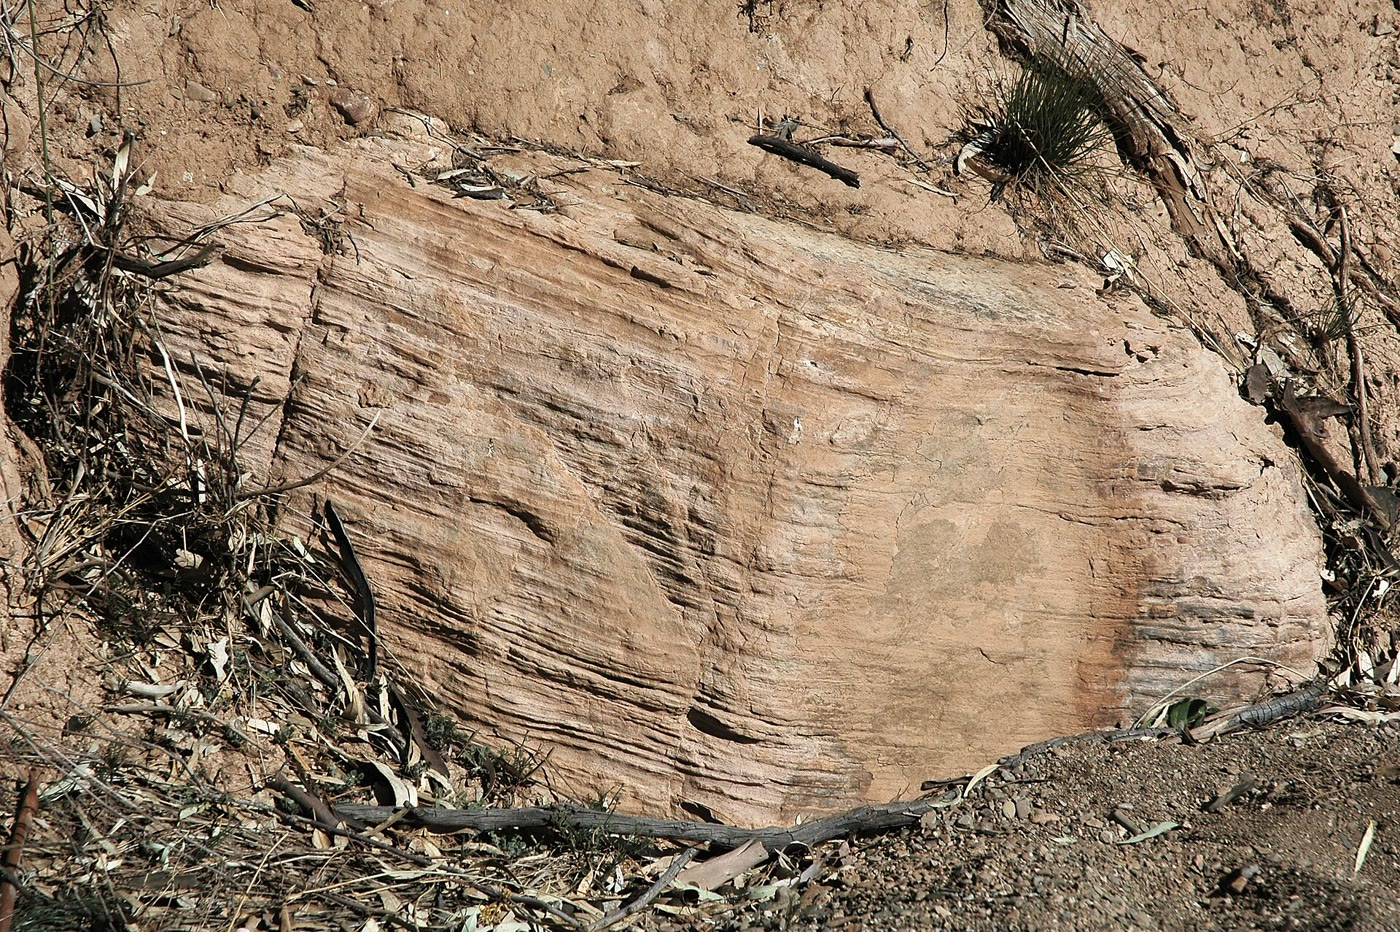
\includegraphics[width=0.66\linewidth]{images/book4/b2-18-cap-carbonate.jpg}
\par\smallskip{\small A \omterm{def:b2:precambrian-earth:snowball}{cap carbonate}: laminated dolostone of the Nuccaleena Formation,
Flinders Ranges, South Australia, resting on the deposits of the Marinoan glaciation
(the beds are tilted). Photograph James St.~John, CC~BY~2.0 (Wikimedia Commons).}
\end{omfigure}

Two snowballs of the Cryogenian are now dated by uranium--lead ages on zircons from volcanic
ash and by rhenium--osmium ages on organic-rich shales. The Sturtian began between 717.5 and
\qty{716.3}{Ma} and ended between 659.3 and \qty{658.5}{Ma}: \qty{58}{Myr} of ice, with the
onset and the end synchronous across the world. The Marinoan began between 649.9 and
\qty{639.0}{Ma}, loosely dated, and ended between 636.0 and \qty{634.7}{Ma}: at least
\qty{3}{Myr}. Each ends with a single \omterm{def:b2:precambrian-earth:snowball}{cap carbonate}, never with several. Iron formations,
absent for a billion years, return in the Sturtian glacial deposits. At least one earlier
snowball, in the Siderian around \qty{2.4}{Ga}, came at the time of the GOE; between the two
episodes, for some \qty{1.5}{Gyr}, almost no ice sheets are known.
% ledger: hoffman17:ages, hoffman17:cryochrons, hoffman17:cap, hoffman17:models, hoffman17:earlier

\begin{history}[From an odd hypothesis to a dated theory]
In 1964 W.~B. Harland drew attention to the evidence for a late Precambrian glaciation. In
1968 and 1969 M.~I. Budyko, and W.~D. Sellers with a similar model, found that the
\omterm{def:b2:precambrian-earth:ice-albedo}{ice--albedo feedback} could make the ice spread to the equator once it advanced far enough; a
globally frozen Earth then seemed a state without return, and so one that had never happened.
In 1981 J.~Walker, P.~Hays and J.~Kasting described the thermostat of silicate weathering and
noted that on a frozen Earth the carbon dioxide of volcanoes would accumulate until the ice
melted: the state could end itself. In 1992 J.~L. Kirschvink proposed that it had in fact
happened, and named it the ``\omterm{def:b2:precambrian-earth:snowball}{Snowball Earth}''; in 1998 P.~F. Hoffman and colleagues published
``A Neoproterozoic \omterm{def:b2:precambrian-earth:snowball}{Snowball Earth}'', and the panglacial epochs came to be called cryochrons. No
Cryogenian glacial deposit had been dated radiometrically before 2004; the dates above are the
work of the years since.
\end{history}
% ledger: hoffman17:history

Volcanoes are the way out. On an Earth covered in ice, rain and rivers almost stop, silicate
weathering with them, and the carbon dioxide that volcanoes release accumulates in the air
until its greenhouse melts the ice.

\begin{proposition}[Carbon dioxide build-up]\label{prop:b2:precambrian-earth:co2}
If carbon dioxide is released at a rate $F$ (mass per year) into an atmosphere of mass
$M_{\text{a}}$ and mean molar mass $\bar M$, with no sink, the time needed to bring its volume
mixing ratio from nearly zero to $x$ is
\[
  \tau = \frac{x}{1 - x}\,\frac{M_{\mathrm{CO_2}}}{\bar M}\,\frac{M_{\text{a}}}{F} .
\]
\end{proposition}

\begin{proof}
The atmosphere holds $n = M_{\text{a}}/\bar M$ moles of other gases. Adding $n_c$ moles of
carbon dioxide makes its mixing ratio $x = n_c/(n + n_c)$, so $n_c = n\,x/(1 - x)$, of mass
$n_c M_{\mathrm{CO_2}}$; at the rate $F$ this takes $\tau = n_c M_{\mathrm{CO_2}}/F$.
\end{proof}

\begin{example}[How long to escape?]\label{ex:b2:precambrian-earth:escape}
The highest preferred estimate of today's volcanic release is \qty{0.26}{Gt} of carbon
dioxide a year. Estimates of the
mixing ratio needed to end a Cryogenian snowball range from 0.01 to 0.1. With $M_{\text{a}} =
\qty{5.1e18}{kg}$, $\bar M = \qty{28.97}{g.mol^{-1}}$ and $M_{\mathrm{CO_2}} =
\qty{44.01}{g.mol^{-1}}$, $x = 0.01$ takes $\frac{0.01}{0.99}\times1.519\times\qty{5.1e18}{kg}
/ \qty{0.26e12}{kg.yr^{-1}} = \qty{0.30}{Myr}$, and $x = 0.1$ takes \qty{3.3}{Myr}.
\end{example}
% ledger: usgs:volcanic-co2, hoffman17:co2, earth:Matm, earth:Mmol, ciaaw:abridged-2024
% values: co2_t001_Myr 0.301, co2_t01_Myr 3.311 (precambrian.py)

A column of pure carbon dioxide weighing \qty{1}{bar} over the whole Earth would take
\qty{20}{Myr} at the same rate, the figure Walker, Hays and Kasting gave. A few million years
is long, but the Sturtian lasted \qty{58}{Myr}. Either the threshold was higher, or the
outgassing lower, or the frozen Earth still had sinks: the weathering of the young sea floor,
which does not stop under ice, is one candidate. In the energy-balance model the escape needs
the snowball's effective emissivity to fall until its temperature reaches \qty{263}{K}: under
the Cryogenian Sun, \qty{94}{\percent} of today's, from 0.616 to 0.472, an extra trapping of
some \qty{39}{W.m^{-2}} (\cref{exo:b2:precambrian-earth:10}).
% ledger: hoffman17:co2, hoffman17:models, usgs:volcanic-co2
% values: one_bar_Myr 19.98, eps_melt_094 0.4716, forcing_melt_094 39.1 (precambrian.py)

When the ice finally opens at the equator, the feedback runs backwards: dark sea absorbs more
sunlight, the ice retreats, and the models have the ice line racing to the poles in about
\qty{2}{kyr}. The Earth then finds itself with an enormous greenhouse on a dark surface, a hot
aftermath. Weathering, very fast in that climate, pours calcium, magnesium and bicarbonate into
the sea, where the \omterm{def:b2:precambrian-earth:snowball}{cap carbonates} precipitate while the meltwater floods the shelves; it takes
some ten million years to draw the carbon dioxide back down. The ice sheets and the \omterm{def:b2:precambrian-earth:snowball}{cap
carbonates}, the iron formations and the synchronous ages are why most geologists now accept
that the Cryogenian snowballs happened, although how hard they were --- whether a belt of open
water survived at the equator, as ``waterbelt'' models propose --- is still argued.
% ledger: hoffman17:hysteresis, hoffman17:cap, hoffman17:debate

\section*{Exercises}\label{sec:b2:precambrian-earth:exercises}

Data for the exercises, unless stated otherwise: $\sigma = \qty{5.670e-8}{W.m^{-2}.K^{-4}}$;
$S_0 = \qty{1361}{W.m^{-2}}$; today's albedo 0.294 and mean surface temperature \qty{288}{K};
snowball albedo 0.6; ramp from \qty{263}{K} to \qty{283}{K}; effective emissivity today
0.616; Gough's law $L/L_0 = 1/(1 + 0.4\,t/t_\odot)$ for a time $t$ before present, $t_\odot =
\qty{4.567}{Gyr}$; \omterm{def:b2:precambrian-earth:greenstone}{komatiite} liquidus \qty{1616}{\celsius} at \qty{32.2}{\percent} MgO,
slope \qty{18.0}{\celsius} per per cent; half-lives \ce{^{238}U} \qty{4.468}{Gyr}, \ce{^{235}U}
\qty{0.704}{Gyr}, \ce{^{232}Th} \qty{14.0}{Gyr}, \ce{^{40}K} \qty{1.248}{Gyr}.
% ledger: const:sigma, earth:TSI, earth:albedo, earth:Tsurf, hoffman17:models, gough81:luminosity, connelly12:cai, so16:liquidus, iaea:isotopes

\begin{exercise}[$\star$]\label{exo:b2:precambrian-earth:1}
(a) How long did the \omterm{def:b2:precambrian-earth:eons}{Hadean}, the \omterm{def:b2:precambrian-earth:eons}{Archean} and the \omterm{def:b2:precambrian-earth:eons}{Proterozoic} last? (b) What fraction of the age
of the Earth do the three together make? (c) How old was the Earth when the oldest known zircon
crystallised, and when the oldest rocks formed?
\end{exercise}

\begin{exercise}[$\star$]\label{exo:b2:precambrian-earth:2}
Today the \omterm{def:b2:elements-in-the-earth:bse}{bulk silicate Earth} releases, per kilogram, \qty{1.917}{pW} from \ce{^{238}U},
\qty{0.082}{pW} from \ce{^{235}U}, \qty{2.089}{pW} from \ce{^{232}Th} and \qty{0.818}{pW} from
\ce{^{40}K} ($\qty{1}{pW} = \qty{e-12}{W}$). (a) Find each contribution \qty{3}{Gyr} ago, and
the total. (b) By what factor has the heat production fallen since? (c) Which isotope leads
today, and which led then?
\end{exercise}

\begin{exercise}[$\star$]\label{exo:b2:precambrian-earth:3}
Use the \omterm{def:b2:precambrian-earth:greenstone}{komatiite} thermometer. (a) What is the liquidus of a \omterm{def:b2:precambrian-earth:greenstone}{komatiite} with
\qty{28}{\percent} MgO? (b) What MgO content corresponds to \qty{1500}{\celsius}? (c) A
spinifex-textured flow has a whole-rock MgO of \qty{38}{\percent}. Why should its liquidus not
be read from the line?
\end{exercise}

\begin{exercise}[$\star$]\label{exo:b2:precambrian-earth:4}
Put the following in order and give their approximate ages: the \omterm{def:b2:precambrian-earth:goe}{Great Oxidation Event}, the
first stromatolites, the end of the Marinoan glaciation, the last common \omterm{def:b2:precambrian-earth:greenstone}{komatiites}, the
oldest rocks, the second rise of oxygen, the first Ediacaran fossils, the end of the dome-and-keel
structures of the Pilbara.
\end{exercise}

\begin{exercise}[$\star\star$]\label{exo:b2:precambrian-earth:5}
(a) Check that the effective emissivity of today's Earth is 0.616. (b) Find the snowball
equilibrium under today's Sun. (c) Show that the middle equilibrium, \qty{275.5}{K}, satisfies
$R = E$ to within \qty{0.5}{W.m^{-2}}. (d) Find the slopes of $R$ and $E$ there, and conclude
that it is unstable.
\end{exercise}

\begin{exercise}[$\star\star$]\label{exo:b2:precambrian-earth:6}
(a) Using Gough's law, find the sunlight \qty{2.4}{Ga} ago and \qty{0.65}{Ga} ago as fractions
of today's. (b) In the model, is a warm climate possible at each date with today's emissivity?
(c) Hoffman and colleagues write that the Siderian Sun was about \qty{10}{\percent} dimmer than
the Cryogenian Sun. Check.
\end{exercise}

\begin{exercise}[$\star\star$]\label{exo:b2:precambrian-earth:7}
The Sturtian lasted from \qty{716.9}{Ma} to \qty{658.9}{Ma} (middles of the dated intervals),
the Marinoan from \qty{644.5}{Ma} to \qty{635.4}{Ma}. (a) Find their durations and the
interglacial between them. (b) What fraction of the Cryogenian period, 720 to \qty{635}{Ma},
did ice cover the Earth, on these figures? (c) Why is the duration of the Marinoan only a
rough figure?
\end{exercise}

\begin{exercise}[$\star\star$]\label{exo:b2:precambrian-earth:8}
(a) How long does it take volcanoes, at \qty{0.26}{Gt} a year with no sink, to bring the air to
a carbon dioxide mixing ratio of 0.05? (b) How many times the \qty{278}{ppm} of 1750 is that? (c) If half of the release were taken up by the weathering of the sea
floor, how long would it take?
\end{exercise}
% ledger: usgs:volcanic-co2, earth:Matm, earth:Mmol, ciaaw:abridged-2024, ipcc:erf-2xco2

\begin{exercise}[$\star\star$]\label{exo:b2:precambrian-earth:9}
A Neoproterozoic diamictite contains striated stones, some of which lie in finely laminated mud
that is bent down beneath them. (a) What does the bending tell? (b) Its palaeolatitude is
\ang{10}. Why does this matter for the snowball hypothesis? (c) It is directly overlain by a
pink laminated dolostone a few metres thick. What is it, and what does it record?
\end{exercise}

\begin{exercise}[$\star\star\star$]\label{exo:b2:precambrian-earth:10}
Under the Cryogenian Sun, $S = 0.94\,S_0$. (a) Show that in the model the warm state still
exists, barely, but that a snowball also exists. (b) Find the snowball's temperature with
today's emissivity. (c) Find the emissivity at which the snowball reaches \qty{263}{K} and
thaws. (d) Convert the change of emissivity into an extra trapping of longwave radiation at
\qty{263}{K}, in \unit{W.m^{-2}}.
\end{exercise}

\begin{exercise}[$\star\star\star$]\label{exo:b2:precambrian-earth:11}
(a) Using the tipping points of \cref{prop:b2:precambrian-earth:tipping}, show that the width
of the hysteresis loop, $S_{\text{m}}/S_{\text{f}}$, does not depend on the emissivity, and
compute it. (b) What would make the loop narrower? (c) Why can a snowball thaw only far from
the conditions in which it froze?
\end{exercise}

\begin{exercise}[$\star\star\star$]\label{exo:b2:precambrian-earth:12}
Derive the time constant of the energy-balance model near the warm equilibrium, $\tau =
C/(E'(T^*) - R'(T^*))$, and evaluate it for an ocean mixed layer \qty{50}{m} deep, of density
\qty{1025}{kg.m^{-3}} and specific heat \qty{3992}{J.kg^{-1}.K^{-1}}. What happens to $\tau$ as the
sunlight approaches the left tipping point, in this model and in a model whose albedo varies
smoothly with temperature?
\end{exercise}
% ledger: noaa:seawater-1025, teos10:cp0

\begin{problem}[{Weekend problem --- A hotter young Earth}]\label{pb:b2:precambrian-earth:1}
This problem follows the young Earth from its interior to its air. Use the data of the
exercises; the \omterm{def:b2:elements-in-the-earth:bse}{bulk silicate Earth} holds \qty{0.0203}{ppm} of uranium, \qty{0.0795}{ppm} of
thorium and \qty{240}{ppm} of potassium by mass, and its isotopes release \qty{95.13}{\micro W}
(\ce{^{238}U}), \qty{568.47}{\micro W} (\ce{^{235}U}), \qty{26.28}{\micro W} (\ce{^{232}Th}) and
\qty{28.47}{\micro W} (\ce{^{40}K}) per kilogram of isotope. By mass, uranium is
\qty{99.29}{\percent} \ce{^{238}U} and \qty{0.711}{\percent} \ce{^{235}U}, and potassium
\qty{0.0120}{\percent} \ce{^{40}K}. Round to three significant figures.

\noindent\textbf{Part I --- Heat from inside.}
\begin{enumerate}
  \item Find the heat released today by each isotope per kilogram of \omterm{def:b2:elements-in-the-earth:bse}{bulk silicate Earth}, in
        \unit{pW.kg^{-1}}.
  \item Find the total.
  \item Find the decay constant of each isotope, in \unit{Gyr^{-1}}.
  \item Find each contribution \qty{2.7}{Gyr} ago, when the \omterm{def:b2:precambrian-earth:greenstone}{komatiites} of Pyke Hill erupted.
  \item Find the total then, and the ratio to today's.
  \item Which isotope gave most heat then? Why does it give so little today?
\end{enumerate}

\noindent\textbf{Part II --- The Sun of the Archean.}
\begin{enumerate}[resume]
  \item With Gough's law, find the sunlight \qty{2.7}{Ga} ago as a fraction of today's, and in
        \unit{W.m^{-2}}.
  \item Find the warm equilibrium at that sunlight with today's emissivity. Is it a valid warm
        state of the model?
  \item Find the snowball equilibrium at that sunlight.
  \item What effective emissivity would keep the Earth at \qty{288}{K} with the warm albedo?
  \item Carbon dioxide alone could have done it at 0.004 to \qty{0.03}{bar} at \qty{2.5}{Ga}.
        In an atmosphere of about \qty{1}{bar}, how many times the \qty{278}{ppm} of 1750 is
        that?
  \item Name the process that kept the carbon dioxide at such a level for hundreds of millions
        of years.
\end{enumerate}

\noindent\textbf{Part III --- A snowball and its end.}
\begin{enumerate}[resume]
  \item The first snowball, \qty{2.4}{Ga} ago: find the sunlight then as a fraction of today's.
        Is the warm state of the model still possible with today's emissivity?
  \item At \qty{0.26}{Gt} of carbon dioxide a year, how long does it take to reach a mixing
        ratio of 0.1?
  \item If the threshold under the dimmer Siderian Sun was twice as high, 0.2, how long?
  \item Which rock records the end of a snowball, and how?
  \item Why do the iron formations of the Sturtian need an ocean without oxygen under the ice?
\end{enumerate}

\noindent\textbf{Part IV --- The komatiite thermometer.}
\begin{enumerate}[resume]
  \item Check the slope of the \omterm{def:b2:precambrian-earth:greenstone}{komatiite} line from the two experiments.
  \item A \omterm{def:b2:precambrian-earth:greenstone}{komatiite} liquid of Pyke Hill had \qty{30}{\percent} MgO. Find its liquidus.
  \item Find the liquidus of the Barberton \omterm{def:b2:precambrian-earth:greenstone}{komatiite}, \qty{32.2}{\percent} MgO.
  \item Find the liquidus of a primary ridge basalt with \qty{12}{\percent} MgO.
  \item With the Kilauea slope, \qty{20}{\celsius} per per cent, instead, how hot would the
        basalt be, starting from the Barberton point? How much does the choice of slope matter?
  \item Why is the temperature difference between the two lavas larger than the difference of
        potential temperature between the \omterm{def:b2:precambrian-earth:eons}{Archean} and today's mantle?
  \item To sum up: how much hotter was the hottest \omterm{def:b2:precambrian-earth:eons}{Archean} \omterm{def:b2:precambrian-earth:greenstone}{komatiite} lava than a primary basalt
        of today's ridges?
\end{enumerate}
\end{problem}
% ledger: ms95:pm-trace, dye:isotope-heat, iaea:isotopes, gough81:luminosity, cz20:archean-air, ipcc:erf-2xco2, usgs:volcanic-co2, hoffman17:co2, so16:liquidus, helz98:glass-thermometer, pierru22:komatiite
